% --- [ Performance ] ----------------------------------------------------------

\subsection{Performance}
\label{sec:ver_performance}

The performance characteristics of the various components have been considered during every stage of the development process, but the initial prototypes have prioritised correctness and simplicity over performance. These prototypes have aimed at identifying suitable data structures and algorithms for the problems, through iterative redesigns and reimplementations. Once the major design decisions stabilised, production quality prototypes were being developed and thoroughly tested. To limit the risk of premature optimisations, micro-level performance work was intentionally postponed to the later stages of development.

Components with straight forward implementations (e.g. the LLVM IR library) have been profiled to identify performance bottle necks, as further described in section~\ref{sec:ver_profiling}. When estimating the time complexity of various subgraph isomorphism search algorithms however, algorithm research and the use of intuition proved far more valuable. One of the first throw-away prototypes provided a partial implementation of the subgraph isomorphism algorithm proposed by Ullman. After further research the prototype was eventually discarded as the Ullman algorithm had been proven to scale poorly for randomly connected graphs with more than 700 nodes~\cite{iso_performance_comparison}. To put this into perspective, the \texttt{main} function of the c4\footnote{C in four functions: \url{https://github.com/rswier/c4}} compiler consists of 248 basic blocks; in other words, the CFG of the \texttt{main} function is a connected graph (every node is reachable from the entry node) with 248 nodes. This leaves a margin (for the number of basic blocks in functions) of less than an order of magnitude before the Ullman algorithm starts to perform poorly.

There exist several subgraph isomorphism algorithms which scale better than the Ullman algorithm for graphs with a large number of nodes; such as the VF2 algorithm for dense graphs and McKay's nauty algorithm for sparse graphs~\cite{iso_performance_comparison,subgraph_isomorphism_algorithms}. In the case of the c4 compiler, the CFGs are sparse with $ 1.35 $ edges per node in average, which would favour the nauty algorithm. The specific properties of CFGs (e.g. sparse connected graphs) guided the design of the subgraph isomorphism search algorithm, as further described in section~\ref{sec:impl_subgraph_isomorphism_search_library}.

To stress test the implementation of the decompilation components and to get an estimate of their time complexities, a set of C programs were automatically generated\footnote{Generate nested C programs: \url{https://gist.github.com/mewmew/677994ee8da60bee1de9}} with $ 2^{x} $ nested \texttt{if}-statements (where $ 7 \le x \le 12 $). These C programs were converted to LLVM IR and decompiled into Go using the same steps as described in appendix~\ref{app:clang_example},~\ref{app:control_flow_graph_generation_example},~\ref{app:restructure_example},~\ref{app:code_generation_example} and~\ref{app:post-processing_example}. The time complexity of each step may be estimated by monitoring how the execution time changes with regards to $ n $, where $ n $ represents the number of nodes in the CFG of the generated programs; as summarised in table~\ref{tbl:run_time_summary}. The CFG of each generated program contains exactly twice as many nodes as nested \texttt{if}-statements; i.e. $ n = 2^{x+1} $.

\begin{table}[htbp]
	\begin{center}
		\begin{tabular}{|l|l|l|l|l|l|l|}
			\hline
			Component & $ n = 256 $ & $ n = 512 $ & $ n = 1024 $ & $ n = 2048 $ & $ n = 4096 $ & $ n = 8192 $ \\
			\hline
			% * ll2dot
			%
			%     n= 256:      1.14s ( 0m01.135s,  0m01.168s,  0m01.114s)
			%     n= 512:      4.01s ( 0m04.060s,  0m04.059s,  0m03.897s)
			%     n=1024:     15.27s ( 0m15.057s,  0m15.714s,  0m15.038s)
			%     n=2048:     58.51s ( 0m59.168s,  0m59.675s,  0m56.698s)
			%     n=4096:  3m 55.84s ( 3m59.045s,  3m53.217s,  3m55.250s)
			%     n=8192: 15m 43.88s (15m40.832s, 15m42.877s, 15m47.934s)
			%
			% As the size of n doubles, the execution time roughly quadruples (4).
			\rowcolor{light_green_3}
			\texttt{ll2dot} & 1.14s & 4.01s & 15.27s & 1m 0s & 3m 56s & 15m 44s \\
			% * restructure
			%
			%     n= 256:      0.97s ( 0m00.974s)
			%     n= 512:      4.37s ( 0m04.370s)
			%     n=1024:     21.37s ( 0m21.374s)
			%     n=2048:  2m  6.34s ( 2m06.344s)
			%     n=4096: 11m  0.56s ( 11m0.555s)
			%     n=8192: 85m 58.35s (85m58.345s)
			%
			% As the size of n doubles, the execution time roughly octuples (8).
			\rowcolor{light_green_3}
			\texttt{restructure} & 0.97s & 4.37s & 21.37s & 2m 6s & 11m 1s & 85m 58s \\
			% * ll2go
			%
			%     n= 256:      2.85s ( 0m02.849s)
			%     n= 512:     10.59s ( 0m10.587s)
			%     n=1024:     40.95s ( 0m40.946s)
			%     n=2048:  2m 41.42s ( 2m41.417s)
			%     n=4096: 10m 46.56s (10m46.562s)
			%     n=8192: 45m 13.16s (45m13.161s)
			%
			% As the size of n doubles, the execution time roughly quadruples (4).
			\rowcolor{light_green_3}
			\texttt{ll2go} & 2.85s & 10.59s & 40.95s & 2m 41s & 10m 47s & 45m 13s \\
			\hline
			\multicolumn{7}{|l|}{\texttt{go-post}} \\
			\hline
			% * unresolved
			%
			%     n= 256:  0.09s (0m00.087s, 0m00.085s, 0m00.084s)
			%     n= 512:  0.29s (0m00.306s, 0m00.286s, 0m00.280s)
			%     n=1024:  1.01s (0m01.008s, 0m01.022s, 0m01.007s)
			%     n=2048:  3.70s (0m03.728s, 0m03.669s, 0m03.703s)
			%     n=4096: 13.87s (0m13.915s, 0m13.771s, 0m13.920s)
			%     n=8192: 53.35s (0m53.265s, 0m53.484s, 0m53.305s)
			%
			% As the size of n doubles, the execution time roughly quadruples (4).
			\rowcolor{light_green_3}
			\textit{unresolved} & 0.09s & 0.29s & 1.01s & 3.70s & 13.87s & 53.35s \\
			% * mainret
			%
			%     n= 256:  0.09s (0m00.084s, 0m00.084s, 0m00.086s)
			%     n= 512:  0.28s (0m00.270s, 0m00.279s, 0m00.276s)
			%     n=1024:  1.00s (0m01.000s, 0m00.997s, 0m01.011s)
			%     n=2048:  3.70s (0m03.658s, 0m03.764s, 0m03.678s)
			%     n=4096: 13.91s (0m13.891s, 0m13.926s, 0m13.900s)
			%     n=8192: 52.91s (0m53.045s, 0m53.029s, 0m52.655s)
			%
			% As the size of n doubles, the execution time roughly quadruples (4).
			\rowcolor{light_green_3}
			\textit{mainret} & 0.09s & 0.28s & 1.00s & 3.70s & 13.91s & 52.91s \\
			% * localid
			%
			%     n= 256:  3m 45.67s ( 3m45.668s)
			%     n= 512: 57m 34.53s (57m34.531s)
			%     n=1024: -
			%     n=2048: -
			%     n=4096: -
			%     n=8192: -
			%
			% The execution time is exponential with regards to n.
			\rowcolor{light_red_3}
			\textit{localid} & 3m 46s & 57m 35s & - & - & - & - \\
			% * assignbinop
			%
			%     n= 256: 0.02s (0m0.015s, 0m0.013s, 0m0.014s)
			%     n= 512: 0.03s (0m0.029s, 0m0.029s, 0m0.028s)
			%     n=1024: 0.07s (0m0.074s, 0m0.073s, 0m0.072s)
			%     n=2048: 0.21s (0m0.213s, 0m0.215s, 0m0.215s)
			%     n=4096: 0.72s (0m0.720s, 0m0.720s, 0m0.719s)
			%     n=8192: 2.63s (0m2.652s, 0m2.613s, 0m2.619s)
			%
			% As the size of n doubles, the execution time roughly quadruples (4).
			\rowcolor{light_green_3}
			\textit{assignbinop} & 0.02s & 0.03s & 0.07s & 0.21s & 0.72s & 2.63s \\
			% * deadassign
			%
			%     n= 256:  0.08s (0m00.078s, 0m00.081s, 0m00.082s)
			%     n= 512:  0.26s (0m00.251s, 0m00.266s, 0m00.263s)
			%     n=1024:  0.95s (0m00.903s, 0m00.999s, 0m00.946s)
			%     n=2048:  3.40s (0m03.372s, 0m03.402s, 0m03.422s)
			%     n=4096: 13.00s (0m12.847s, 0m13.085s, 0m13.078s)
			%     n=8192: 49.96s (0m49.448s, 0m50.316s, 0m50.128s)
			%
			% As the size of n doubles, the execution time roughly quadruples (4).
			\rowcolor{light_green_3}
			\textit{deadassign} & 0.08s & 0.26s & 0.95s & 3.40s & 13.00s & 49.96s \\
			% * forloop
			%
			%     n= 256: 0.01s (0m0.012s, 0m0.012s, 0m0.013s)
			%     n= 512: 0.03s (0m0.038s, 0m0.024s, 0m0.035s)
			%     n=1024: 0.06s (0m0.057s, 0m0.055s, 0m0.054s)
			%     n=2048: 0.15s (0m0.150s, 0m0.149s, 0m0.147s)
			%     n=4096: 0.45s (0m0.455s, 0m0.457s, 0m0.451s)
			%     n=8192: 1.63s (0m1.631s, 0m1.633s, 0m1.640s)
			%
			% As the size of n doubles, the execution time roughly quadruples (4).
			%
			% FUTURE NOTE: Re-run the test with 2^x nested for-loops.
			\rowcolor{light_green_3}
			\textit{forloop} & 0.01s & 0.03s & 0.06s & 0.15s & 0.45s & 1.63s \\
			\hline
		\end{tabular}
	\end{center}
	\caption{The first column specifies the component being tested, and each consecutive column presents the execution time of the component (based on the average of three consecutive runs) in relation to $ n $, which represents the number of nodes in the CFG. Each row below the \texttt{go-post} component represents a specific post-processing rewrite rule (e.g. \textit{mainret}), as further described in appendix~\ref{app:post-processing_example}. The steps which execute in polynomial time with regards to $ n $ have been highlighted in green, while the steps which execute in exponential time with regards to $ n $ have been highlighted in red.}
	\label{tbl:run_time_summary}
\end{table}

Each step of the decompilation pipeline completed in reasonable time (i.e. polynomial time with regards to $ n $) except for one, namely the \textit{``localid''} rewrite rule (see figure~\ref{fig:rewrite_3} of appendix~\ref{app:post-processing_example}) of the post-processing stage. As discussed in section~\ref{sec:evaluation}, most of the post-processing rewrite rules are considered experimental and the \textit{``localid''} rewrite rule suffers from both inaccuracy and performance issues. The \textit{``localid''} rewrite rule optionally provides rudimentary expression propagation support, and will be removed when proper data flow analysis has been implemented by the middle-end (see section~\ref{sec:con_design_validation}).

As the size of $ n $ doubles in table~\ref{tbl:run_time_summary}, the execution time of \texttt{ll2dot} roughly quadruples. The time complexity of \texttt{ll2dot} is therefore estimated to be $ \Omega(n^{2}) $. Please note that this may not hold true for larger values of $ n $, as a formal time complexity analysis of the algorithm is yet to be conducted. Similarly, as the size of $ n $ double, the execution time of \texttt{restructure} roughly octuples. The time complexity of \texttt{restructure} is therefore estimated to be $ \Omega(n^{3}) $. The same logic and caveats may be applied to the other components to estimate their time complexities; a summary of which is presented below.

\begin{itemize}
	\item \texttt{ll2dot}: $ \Omega(n^{2}) $
	\item \texttt{restructure}: $ \Omega(n^{3}) $
	\item \texttt{ll2go}: $ \Omega(n^{2}) $
	\item \texttt{go-post}
	\begin{itemize}
		\item \textit{unresolved}: $ \Omega(n^{2}) $
		\item \textit{mainret}: $ \Omega(n^{2}) $
		\item \textit{localid}: exponential time complexity
		\item \textit{assignbinop}: $ \Omega(n^{2}) $
		\item \textit{deadassign}: $ \Omega(n^{2}) $
		\item \textit{forloop}: $ \Omega(n^{2}) $
	\end{itemize}
\end{itemize}

In summary, profiling is great for optimising the implementations of simple problems. Algorithm research, time complexity theory and intuition is essential for implementing performant solutions to complex problems. Furthermore, knowledge about specific properties of the problem may be exploited to design performant algorithms.

% --- [ Subsubsections ] -------------------------------------------------------

% ~~~ [ Profiling ] ~~~~~~~~~~~~~~~~~~~~~~~~~~~~~~~~~~~~~~~~~~~~~~~~~~~~~~~~~~~~

\subsubsection{Profiling}
\label{sec:ver_profiling}

The initial implementation of the LLVM IR lexer (see section \ref{sec:impl_llvm_ir_library}) focused on correctness, and strived to be as simple and straight forward as possible. Once feature complete and thoroughly tested, the lexer was profiled for the first time and a major performance bottleneck was identified; as illustrated in figure \ref{fig:lexer_pprof}. When scanning letters, the \texttt{lexLetter} function used a hash map to check if the scanned letters were part of a keyword. As letters make up the majority of the characters in LLVM IR source files, this caused an extensive number of hash map iterations which accounted for roughly 70\% of the total execution time. To fix this issue, a benchmark test was implemented to measure the performance changes between the original and the updated version; as further described in section \ref{sec:ver_benchmarks}. At this stage, only CPU profiling has been utilized to identify performance bottlenecks. Future work may leverage memory profiling to further improve the performance of the decompilation components.

\begin{figure}[htbp]
	\begin{center}
		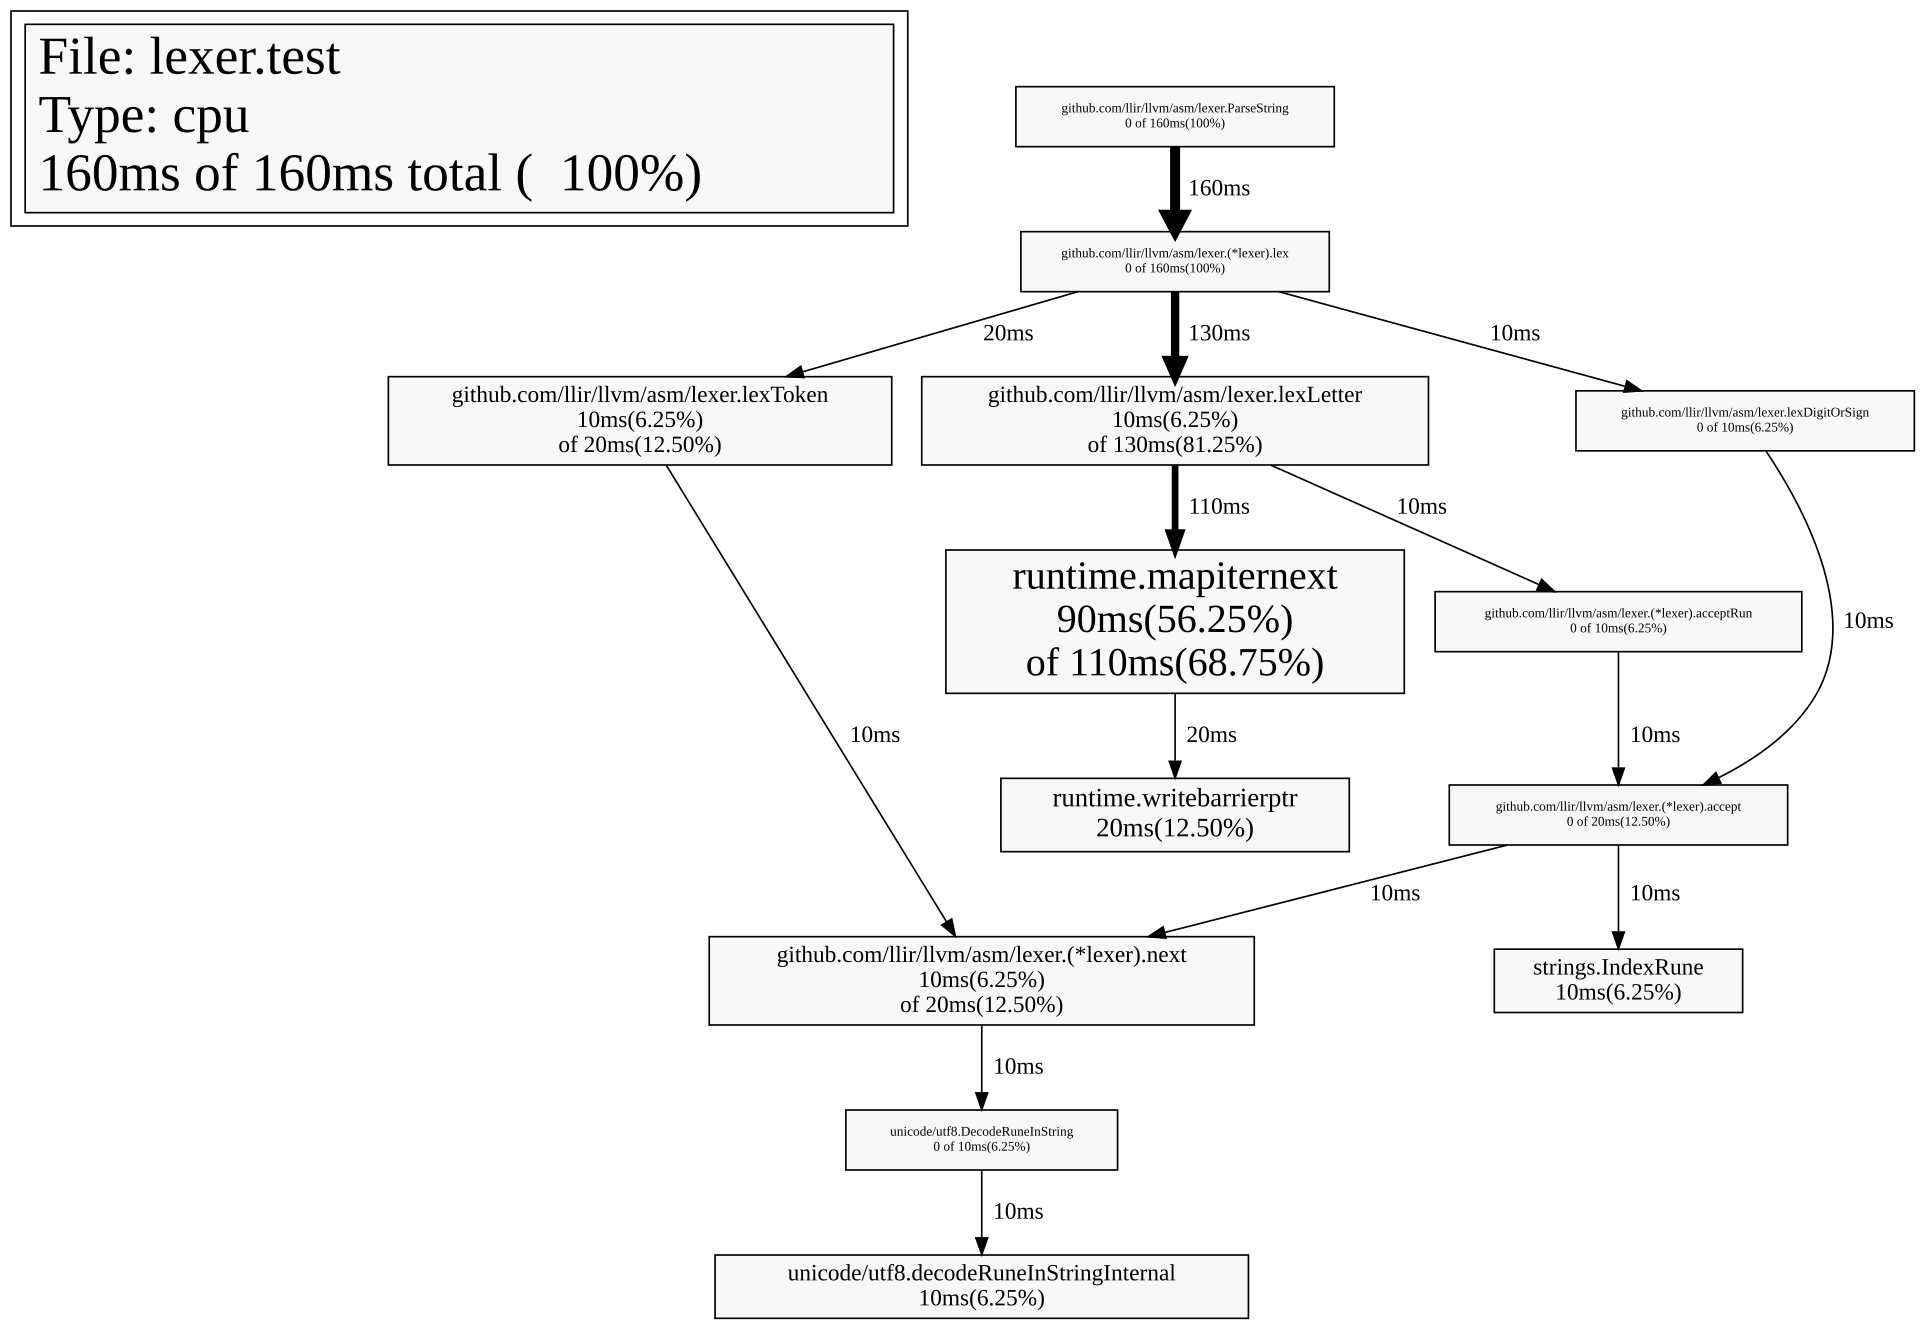
\includegraphics[width=\textwidth]{inc/8_ver/lexer_pprof.png}
		\caption{A major performance bottleneck was located when profiling the LLVM IR lexer for the first time. Roughly 70\% of the total execution time was spent doing hash map iterations (i.e. \texttt{runtime.mapiternext}).}
		\label{fig:lexer_pprof}
	\end{center}
\end{figure}

% ~~~ [ Benchmarks ] ~~~~~~~~~~~~~~~~~~~~~~~~~~~~~~~~~~~~~~~~~~~~~~~~~~~~~~~~~~~

\subsubsection{Benchmarks}
\label{sec:ver_benchmarks}

Benchmark tests were implemented to reliably measure any performance changes before trying to resolve performance issues. An updated version of the LLVM IR library used arrays instead of hash maps to identify keywords when scanning letters, which resolved the performance issue identified in section \ref{sec:ver_profiling}. The updated version of the LLVM IR lexer is roughly 3.6 times faster than the original version, as illustrated in figure \ref{fig:benchmark_delta}.

\begin{figure}[htbp]
	\begin{center}
		\begin{verbatim}
$ git checkout old; go test -bench=ParseString > old.txt
$ git checkout new; go test -bench=ParseString > new.txt
$ benchcmp old.txt new.txt
benchmark                old ns/op     new ns/op     delta
BenchmarkParseString     737625        204010        -72.34%
		\end{verbatim}
		\caption{Benchmark run time delta between the original and the optimized version of the LLVM IR lexer, as visualized by \texttt{benchcmp}\protect\footnotemark. The optimized version is roughly 3.6 times faster than the original vesion of the lexer.}
		\label{fig:benchmark_delta}
	\end{center}
\end{figure}
\footnotetext{Benchcmp displays performance changes between benchmarks: \url{https://golang.org/x/tools/cmd/benchcmp}}

